%This is my super simple Real Analysis Homework template

\documentclass{article}
% \usepackage[utf8]{inputenc}
\usepackage[english]{babel}
\usepackage[]{amsthm} %lets us use \begin{proof}
\usepackage[]{amssymb} %gives us the character \varnothing
\usepackage{amsmath}
\usepackage{geometry}
\usepackage{graphicx}
\graphicspath{ {} }
\geometry{legalpaper, margin=1.2in}
% \usepackage{xeCJK}
% \setCJKmainfont{cwTeXFangSong}
\title{Homework 2}
\author{Chun-Hui,Wu}
\date\today
%This information doesn't actually show up on your document unless you use the maketitle command below

\begin{document}
\maketitle %This command prints the title based on information entered above



\subsection*{Problem 1}
\subsubsection*{1}.Derive the posterior distribution of precision matrix 
\begin{proof}
\begin{eqnarray}
   P(\Lambda | X) & \propto &  P(X|\Lambda)P(\Lambda)\\
   	                                  &\propto& (\frac{|\Lambda|}{2\pi})^{n/2} exp(\sum_{i=1}^n (X_i-\mu)^T\Lambda(X_i-\mu))|\Lambda|^{\frac{n-p-1}{2}}exp(-trace(V^{-1}\Lambda)) \\
                                       &\propto& |\Lambda|^{\frac{2n-p-1}{2}}exp( \sum_{i=1}^n (X_i-\mu)^T\Lambda(X_i-\mu)-trace(V^{-1}\Lambda))\\
                                       &\propto& |\Lambda|^{\frac{2n-p-1}{2}}exp(trace( \sum_{i=1}^n (X_i-\mu)(X_i-\mu)^T-V^{-1})\Lambda )
\end{eqnarray}

For the convenience to derive the MAP , we take log to $P(\Lambda | X)$ then calculate the MAP.
\begin{eqnarray}
   \nabla lnP(\Lambda | X) & \propto & \nabla \frac{2n-p-1}{2}ln|\Lambda| + trace( (\sum_{i=1}^n (X_i-\mu)(X_i-\mu)^T-V^{-1})\Lambda) \\
   	                                  &=& \frac{2n-p-1}{2} \Lambda^{-1} + \sum_{i=1}^n (X_i-\mu)(X_i-\mu)^T-V^{-1} \\
                                       &=& 0\\
\end{eqnarray}

Solve equation 8 ,then we can get MAP.
\begin{eqnarray}
  \Lambda_{MAP}  &= & \frac{2}{2n-p-1} (V^{-1}- \sum_{i=1}^n (X_i-\mu)(X_i-\mu)^T)^{-1}                      
\end{eqnarray}
\end{proof}
\subsubsection*{2}. For N = 10, 100 and 500 calculate $\Lambda_{MAP}$

\[\Lambda_{MAP10}=\begin{bmatrix}
    0.045       & -0.0197   \\
    -0.0197       & 0.0135    \\
\end{bmatrix}\]
\[\Lambda_{MAP100}=\begin{bmatrix}
    0.0006      & -0.00027   \\
    -0.00027       & 0.0002    \\
\end{bmatrix}\]
\[\Lambda_{MAP500}=\begin{bmatrix}
    2.86 * 10^{-5}       & -1.28 *10^{-5}   \\
    -1.28 *  10^{-5}      & 1.029 * 10^{-5}    \\
\end{bmatrix}\]

\clearpage %Gives us a page break before the next section. Optional.
\subsection*{Problem 2}
\subsubsection*{1}Compute the mean vector $m_{N}$ and the covariance matrix $S_{N}$ for the posterior distribution .

\[
m_{N_{10}}= \left[\begin{array}{*{1}c}
0.65 \\
6.56 \\
4.47 \\
-5.19 \\
0.30 \\
-2.70 \\
-12.93 \\
\end{array}\right]
S_{N_{10}}= \left[\begin{array}{*{7}c}
11.75 & -45.13 & 57.52 & -53.28 & 47.82 & -23.10 & 4.99 \\
-45.13 & 186.12 & -243.60 & 226.73 & -203.61 & 98.35 & -21.24 \\
57.52 & -243.60 & 327.17 & -313.87 & 283.55 & -137.05 & 29.60 \\
-53.28 & 226.73 & -313.87 & 318.58 & -293.07 & 142.22 & -30.76 \\
47.82 & -203.61 & 283.55 & -293.07 & 276.29 & -137.93 & 30.41 \\
-23.10 & 98.35 & -137.05 & 142.22 & -137.93 & 74.77 & -19.94 \\
4.99 & -21.24 & 29.60 & -30.76 & 30.41 & -19.94 & 9.08 \\
\end{array}\right]
\]

\[
m_{N_{15}}= \left[\begin{array}{*{1}c}
-1.30 \\
14.94 \\
-7.79 \\
8.32 \\
-12.03 \\
2.84 \\
-13.79 \\
\end{array}\right]
S_{N_{15}}= \left[\begin{array}{*{7}c}
3.91 & -11.81 & 11.80 & -6.62 & 3.75 & -1.46 & 0.53 \\
-11.81 & 44.43 & -49.04 & 27.92 & -15.85 & 6.17 & -2.24 \\
11.80 & -49.04 & 57.72 & -35.46 & 20.71 & -8.11 & 2.95 \\
-6.62 & 27.92 & -35.46 & 26.85 & -17.85 & 7.41 & -2.78 \\
3.75 & -15.85 & 20.71 & -17.85 & 14.85 & -8.77 & 3.96 \\
-1.46 & 6.17 & -8.11 & 7.41 & -8.77 & 10.06 & -6.80 \\
0.53 & -2.24 & 2.95 & -2.78 & 3.96 & -6.80 & 6.25 \\
\end{array}\right]
\]

\[
m_{N_{30}}= \left[\begin{array}{*{1}c}
-1.91 \\
17.13 \\
-9.56 \\
8.02 \\
-10.11 \\
-1.71 \\
-9.89 \\
\end{array}\right]
S_{N_{30}}= \left[\begin{array}{*{7}c}
1.37 & -3.60 & 3.41 & -2.04 & 1.17 & -0.39 & 0.10 \\
-3.60 & 11.94 & -12.90 & 7.90 & -4.55 & 1.54 & -0.40 \\
3.41 & -12.90 & 15.58 & -10.91 & 6.59 & -2.26 & 0.59 \\
-2.04 & 7.90 & -10.91 & 10.32 & -7.44 & 2.80 & -0.77 \\
1.17 & -4.55 & 6.59 & -7.44 & 7.49 & -4.47 & 1.51 \\
-0.39 & 1.54 & -2.26 & 2.80 & -4.47 & 4.73 & -2.54 \\
0.10 & -0.40 & 0.59 & -0.77 & 1.51 & -2.54 & 2.27 \\
\end{array}\right]
\]

\[
m_{N_{80}}= \left[\begin{array}{*{1}c}
0.26 \\
9.39 \\
0.08 \\
0.42 \\
-4.64 \\
-4.21 \\
-9.33 \\
\end{array}\right]
S_{N_{80}}= \left[\begin{array}{*{7}c}
0.42 & -0.78 & 0.52 & -0.27 & 0.14 & -0.07 & 0.02 \\
-0.78 & 1.87 & -1.70 & 0.94 & -0.51 & 0.24 & -0.08 \\
0.52 & -1.70 & 2.19 & -1.71 & 1.05 & -0.51 & 0.18 \\
-0.27 & 0.94 & -1.71 & 2.18 & -1.82 & 0.97 & -0.35 \\
0.14 & -0.51 & 1.05 & -1.82 & 2.19 & -1.59 & 0.64 \\
-0.07 & 0.24 & -0.51 & 0.97 & -1.59 & 1.76 & -0.98 \\
0.02 & -0.08 & 0.18 & -0.35 & 0.64 & -0.98 & 0.80 \\
\end{array}\right]
\]

\subsubsection*{2}.Generate five curve samples from the parameter posterior distribution.

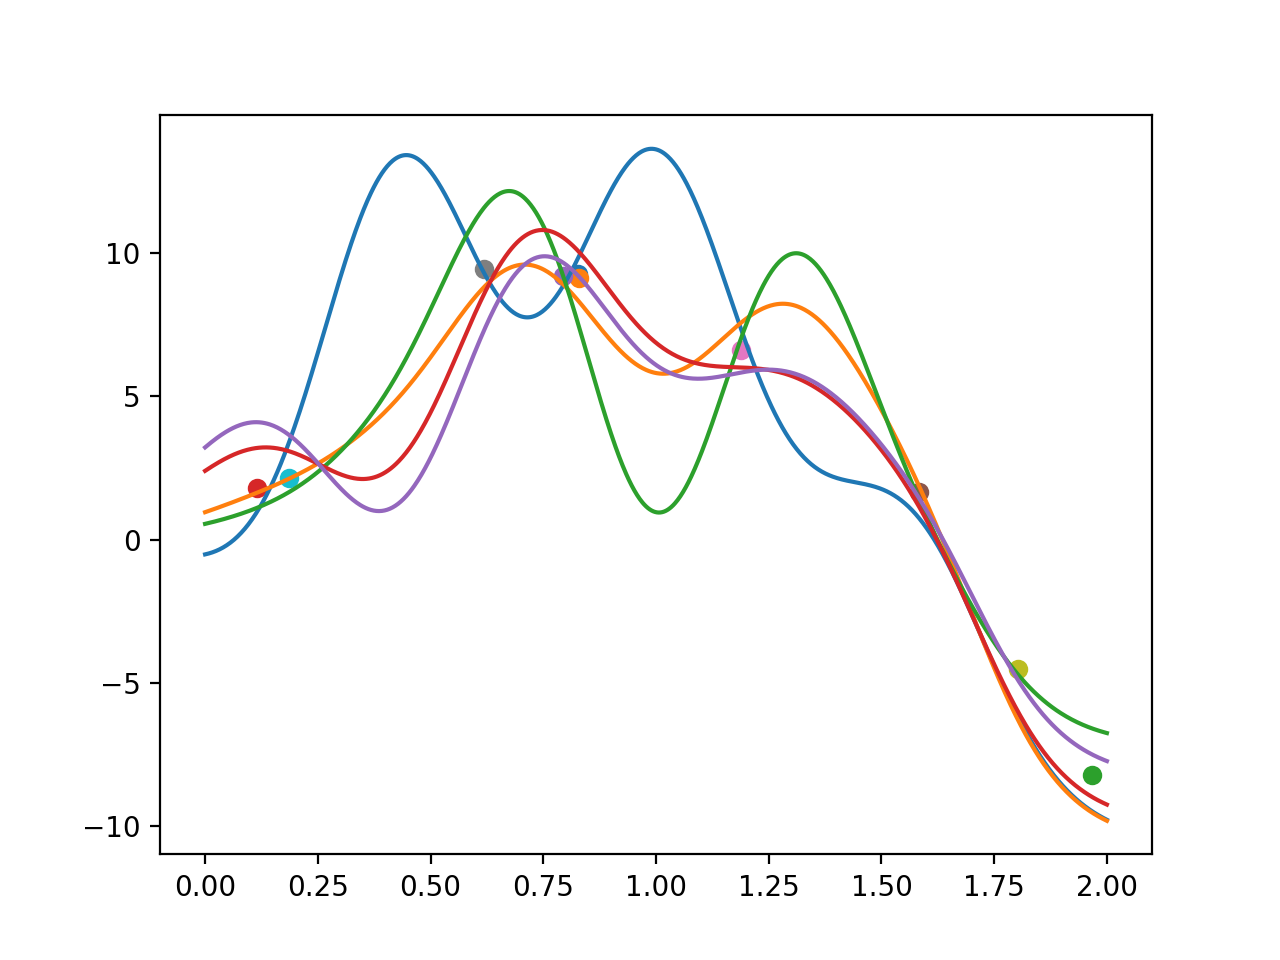
\includegraphics[width=\textwidth]{sample10_5sample.png}\\
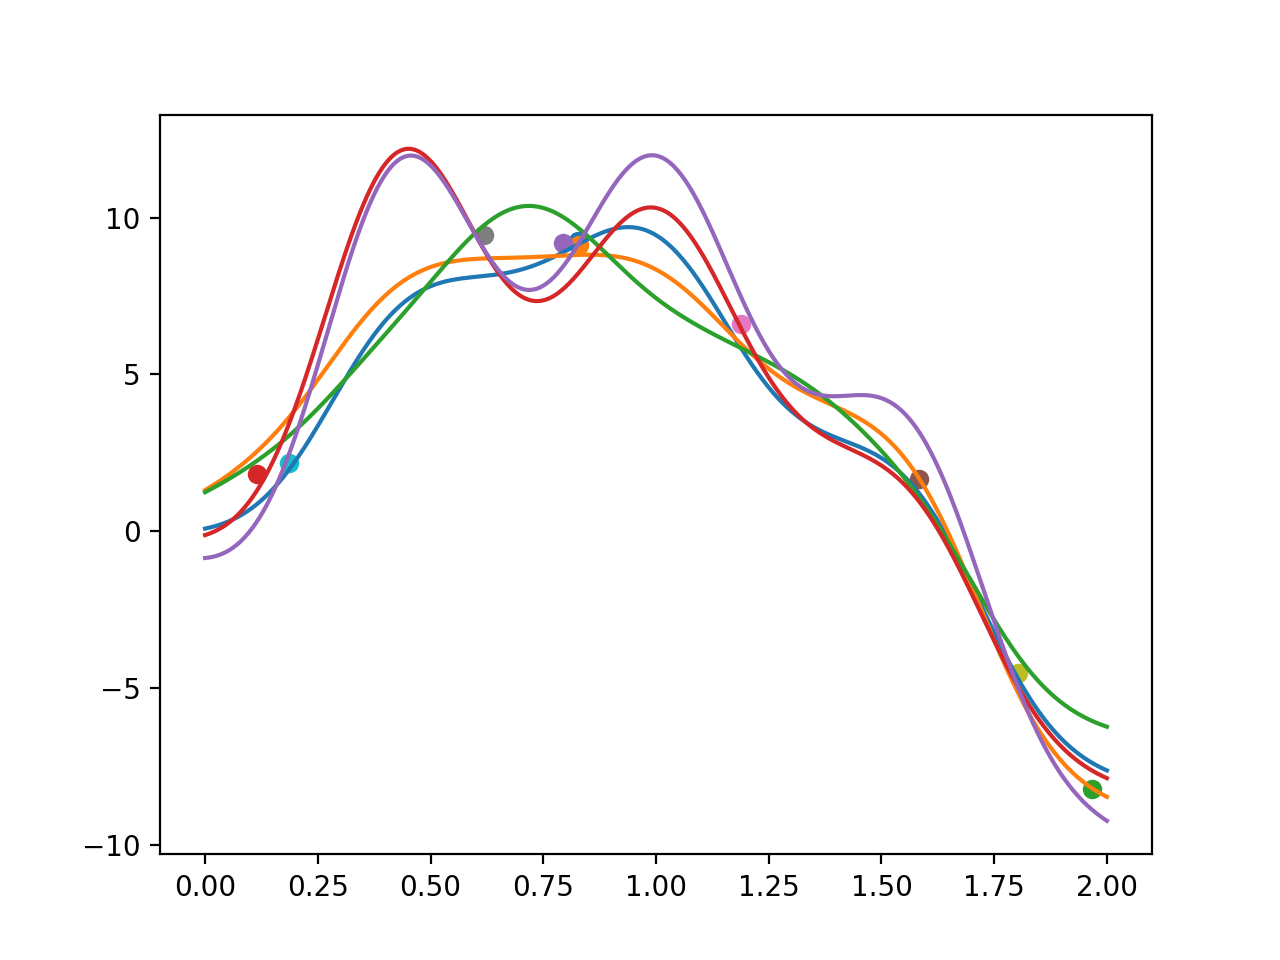
\includegraphics[width=\textwidth]{sample15_sample5.png}\\
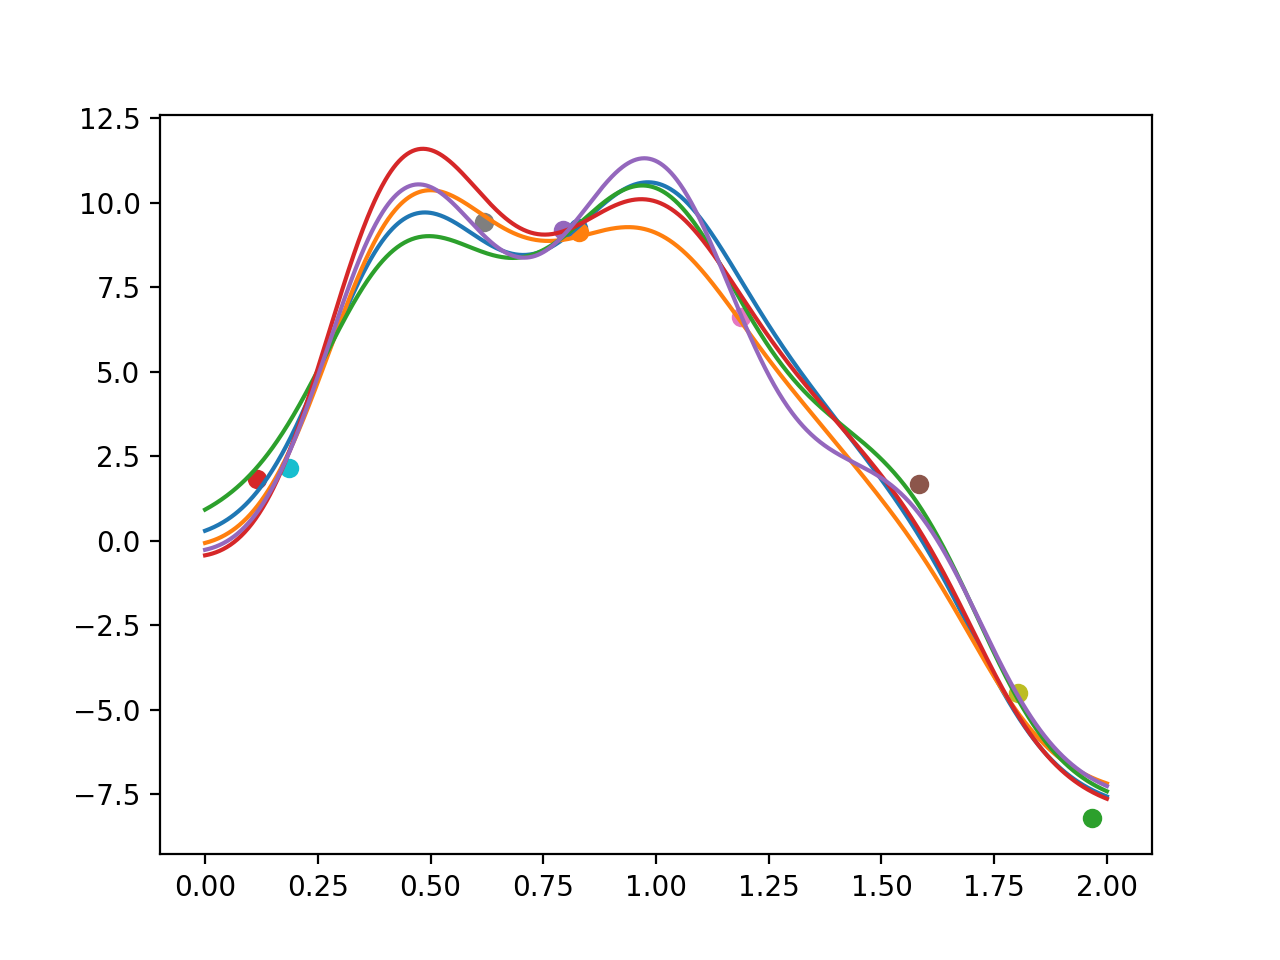
\includegraphics[width=\textwidth]{sample30_sample5.png}\\
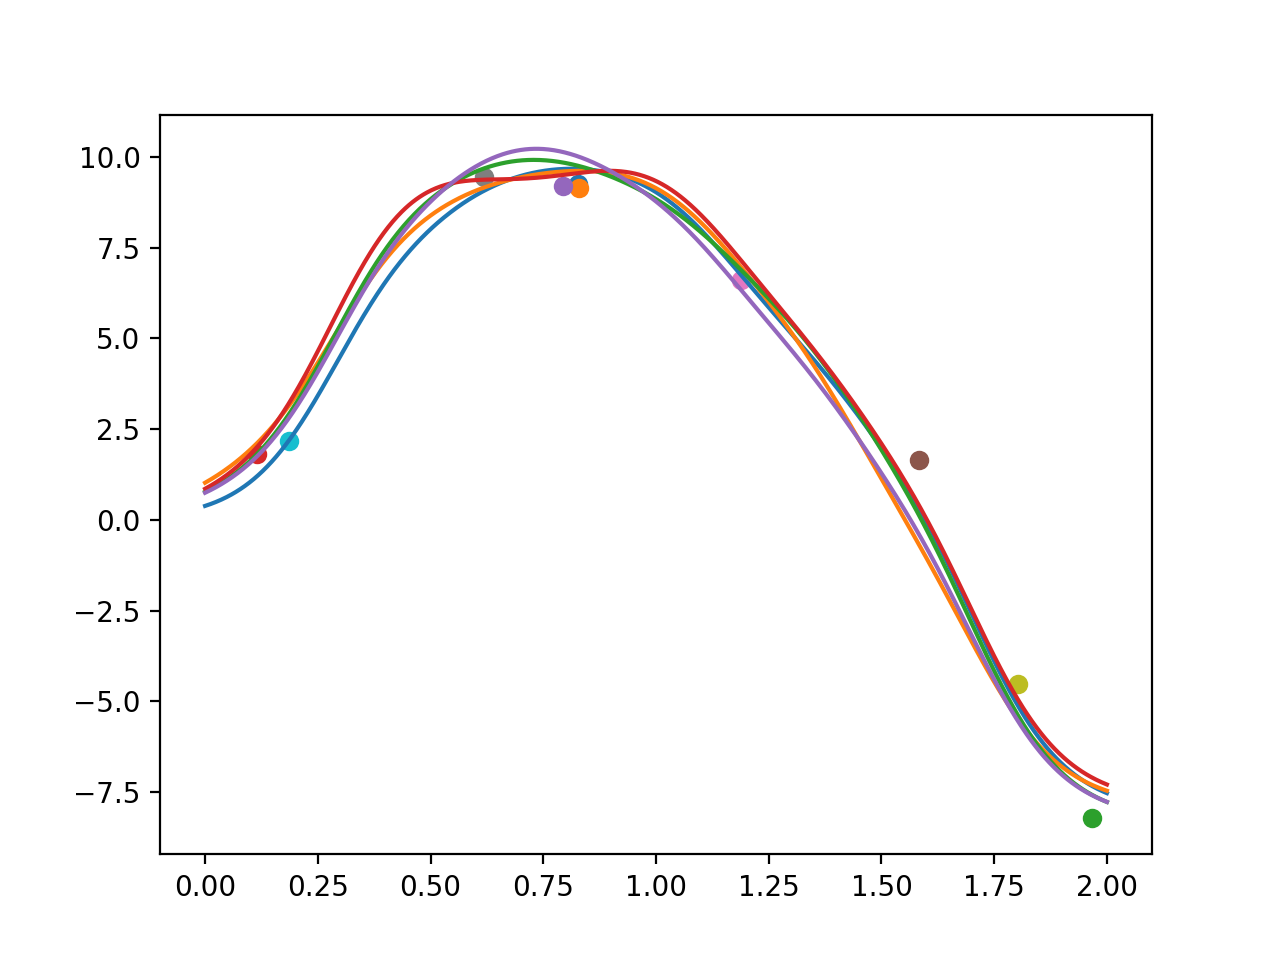
\includegraphics[width=\textwidth]{sample80_sample5.png}\\

As the sample size increase , the sampling result of the posterior become more stable.\\

\subsubsection*{3}.Plot the predictive distribution of target value t and show the mean curve and the region of variance with one standard deviation on either side of the mean curve.

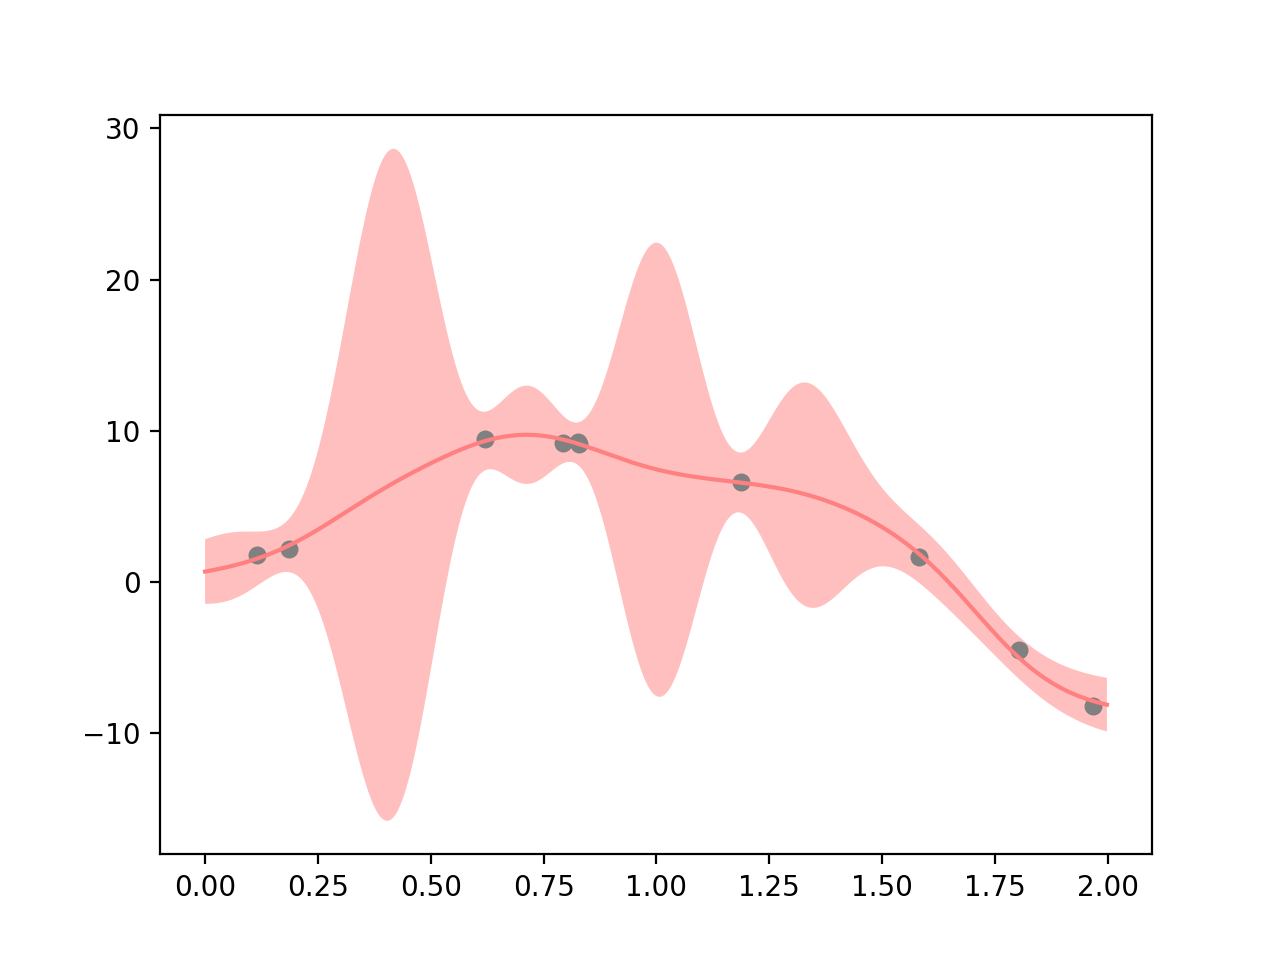
\includegraphics[width=\textwidth]{10sample_predict.png}\\
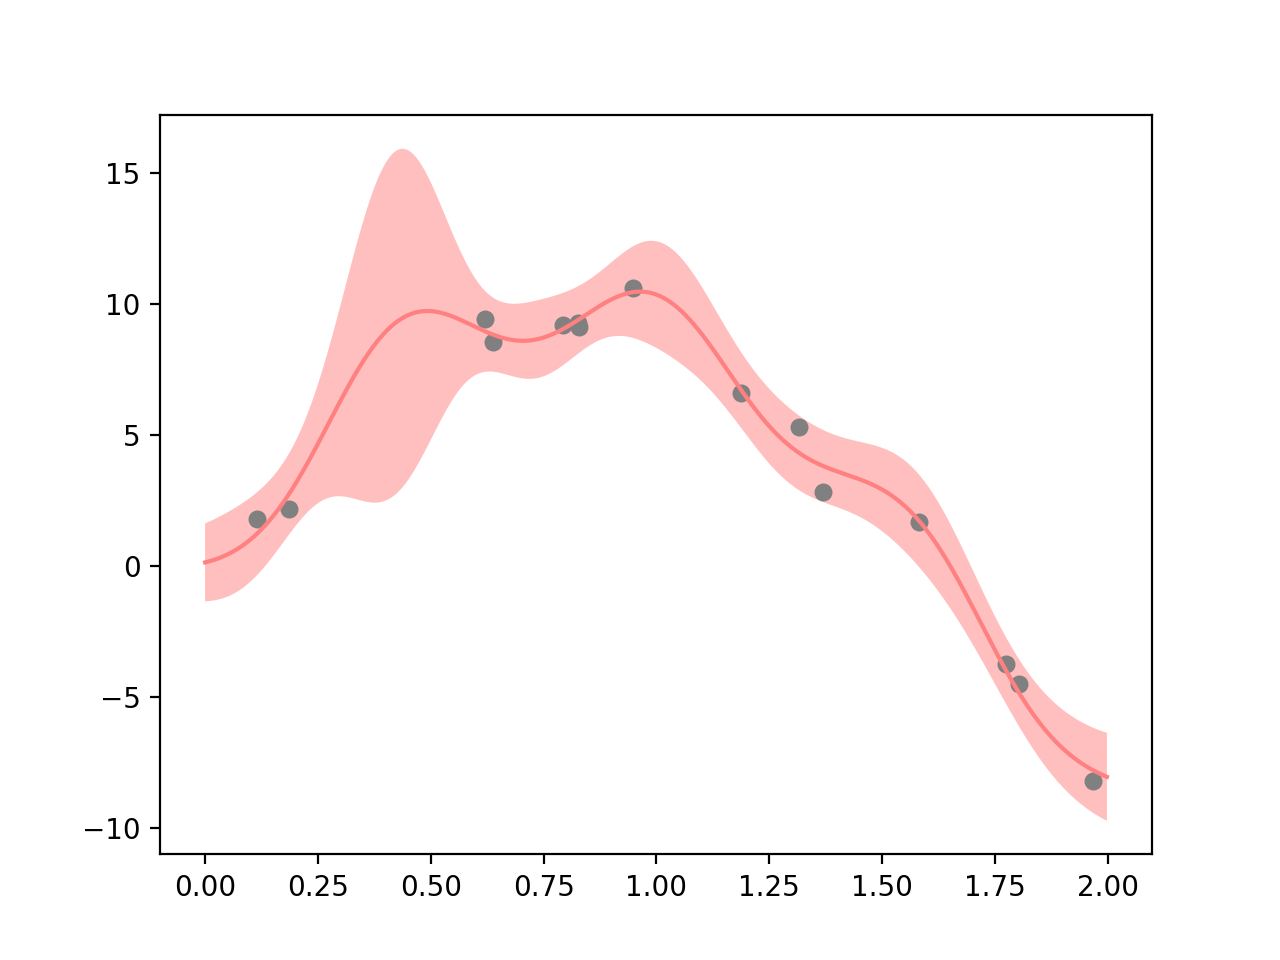
\includegraphics[width=\textwidth]{15sample_predict.png}\\
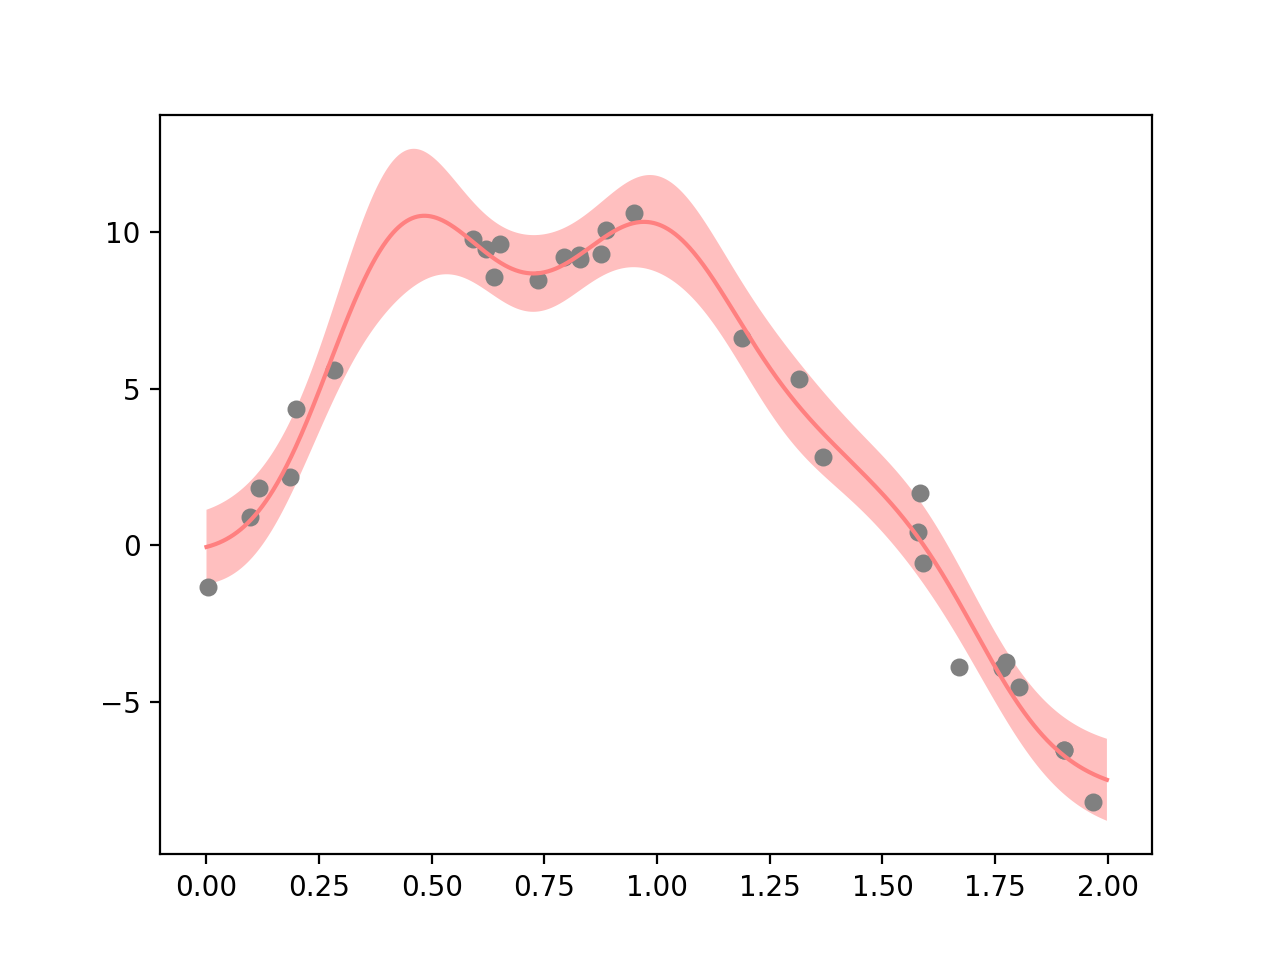
\includegraphics[width=\textwidth]{30sample_predict.png}\\
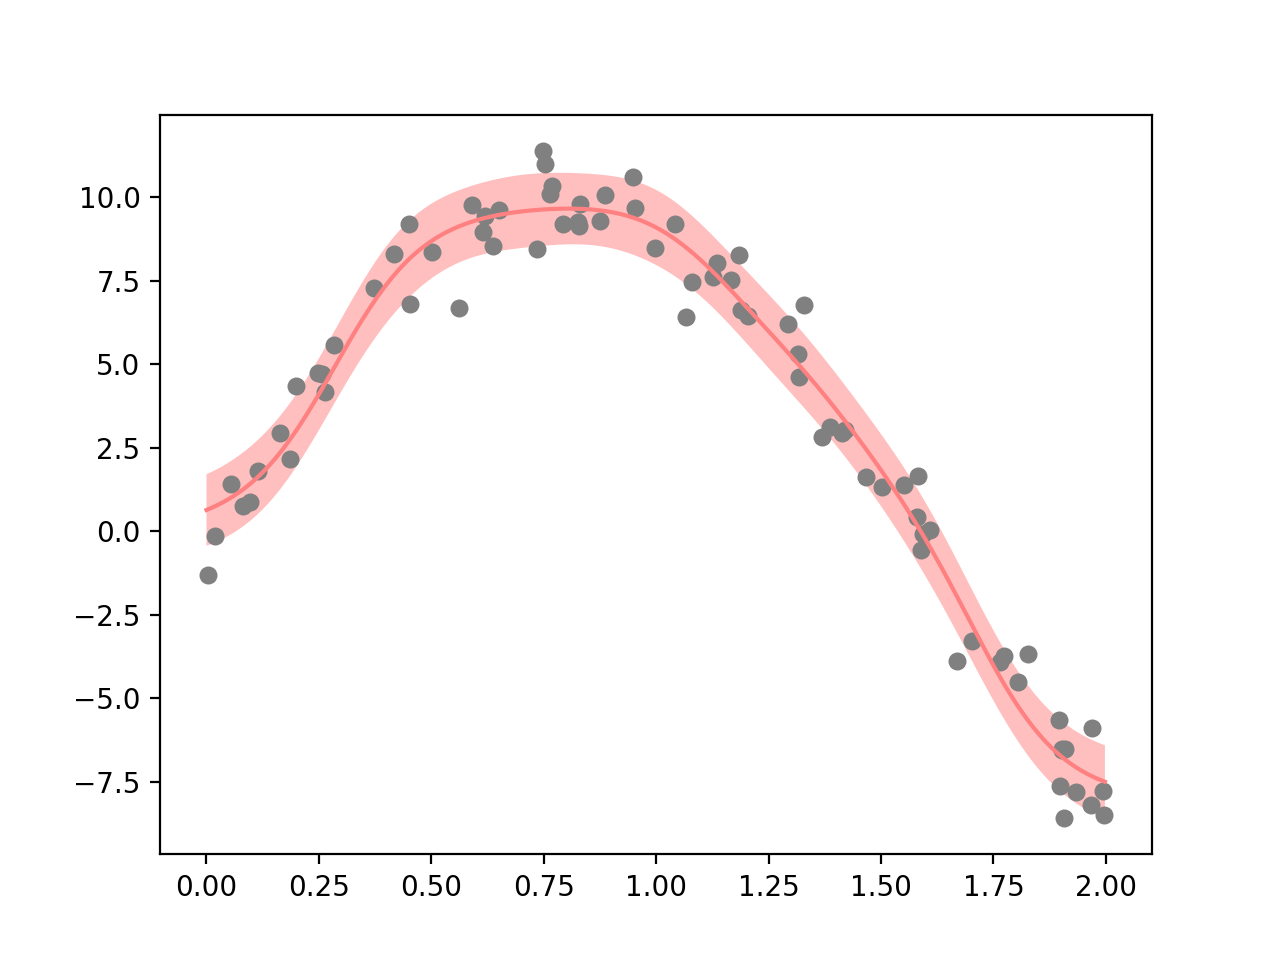
\includegraphics[width=\textwidth]{80sample_predict.png}\\

As the sample size increase , the prediction interval become smaller.

\subsection*{Problem 3}
Implement the Newton-Raphson algorithm to construct a multiclass logistic regression model with the softmax transformation.

\subsubsection*{1}
\subsubsection*{2} Show the classification result of test data.
\[
Y=\begin{bmatrix}
0.00 & 0.00 & 1.00 \\
0.00 & 0.00 & 1.00 \\
0.00 & 0.00 & 1.00 \\
0.00 & 0.00 & 1.00 \\
0.00 & 0.05 & 0.95 \\
0.00 & 0.00 & 1.00 \\
0.00 & 0.00 & 1.00 \\
0.00 & 0.00 & 1.00 \\
0.00 & 0.00 & 1.00 \\
0.00 & 0.00 & 1.00 \\
0.65 & 0.00 & 0.35 \\
0.00 & 0.12 & 0.88 \\
1.00 & 0.00 & 0.00 \\
0.00 & 1.00 & 0.00 \\
0.00 & 1.00 & 0.00 \\
0.00 & 1.00 & 0.00 \\
0.00 & 0.94 & 0.06 \\
0.00 & 1.00 & 0.00 \\
0.00 & 1.00 & 0.00 \\
0.00 & 0.00 & 1.00 \\
1.00 & 0.00 & 0.00 \\
1.00 & 0.00 & 0.00 \\
1.00 & 0.00 & 0.00 \\
1.00 & 0.00 & 0.00 \\
1.00 & 0.00 & 0.00 \\
1.00 & 0.00 & 0.00 \\
1.00 & 0.00 & 0.00 \\
1.00 & 0.00 & 0.00 \\
1.00 & 0.00 & 0.00 \\
1.00 & 0.00 & 0.00 \\
\end{bmatrix}
\]
\subsubsection*{3}Plot the distribution (or histogram) of each variable in training data and map different colors to each class.

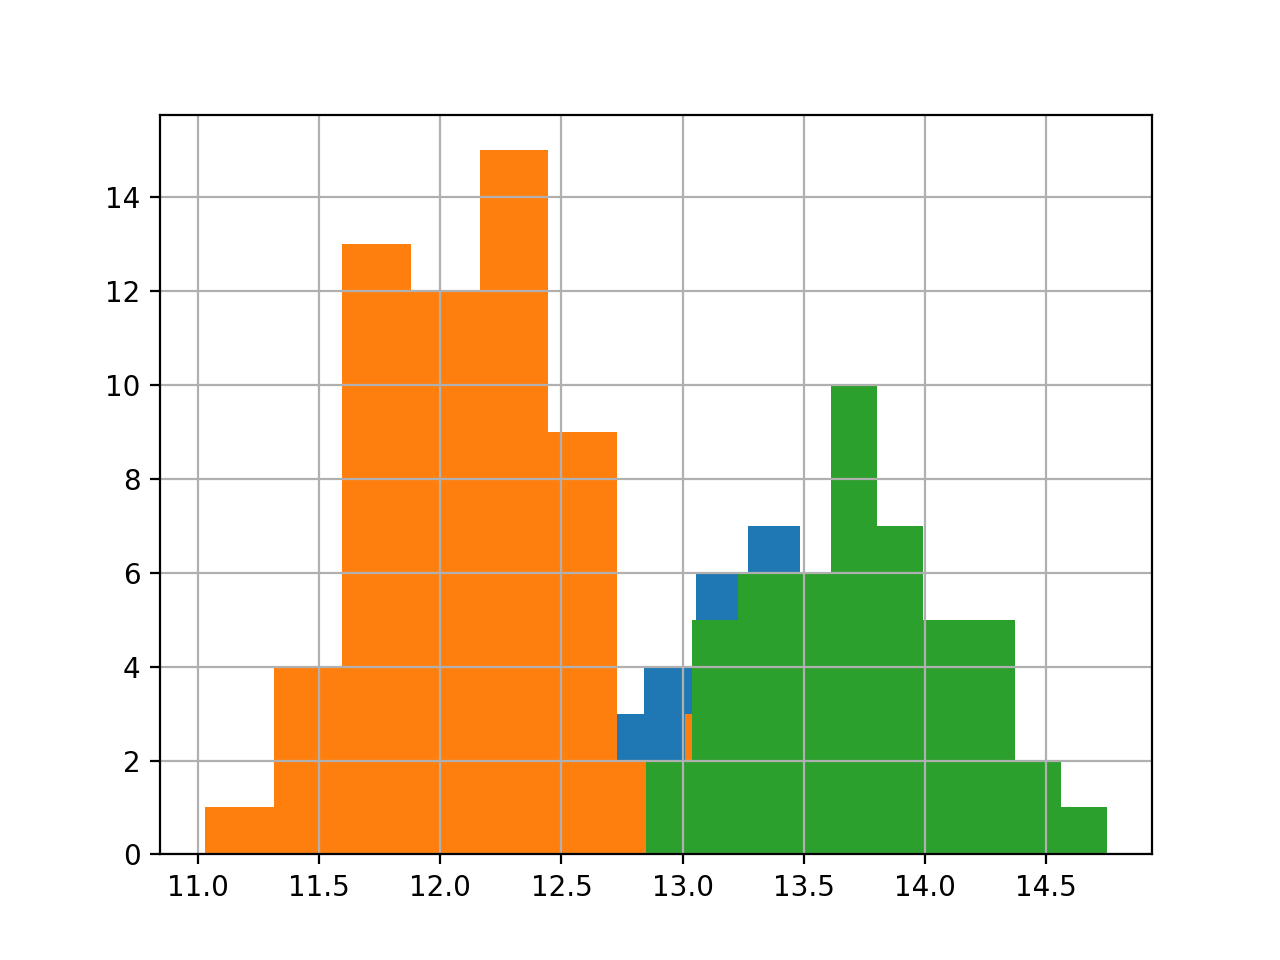
\includegraphics[width=\textwidth]{v1.png}\\
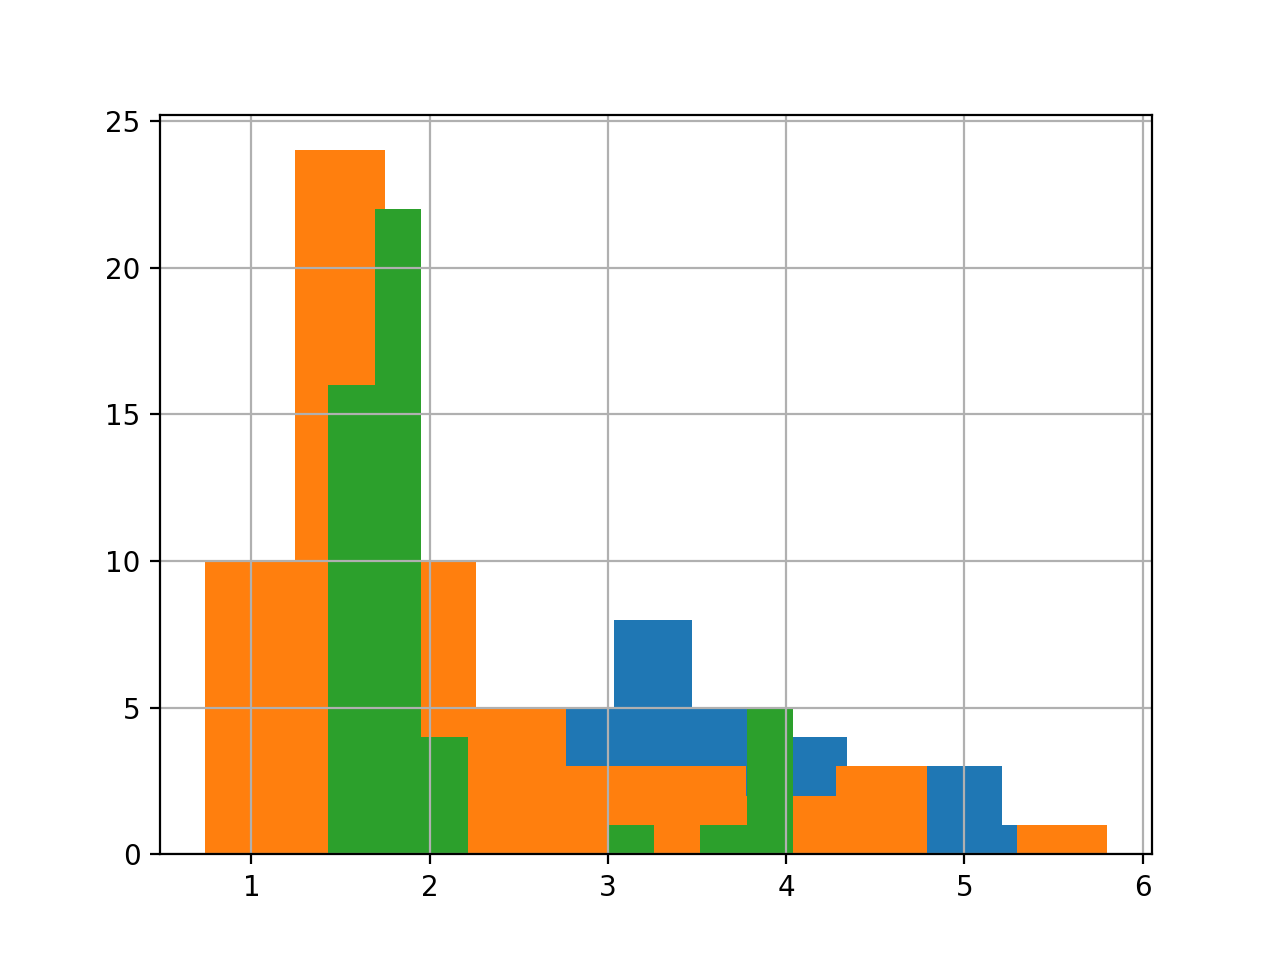
\includegraphics[width=\textwidth]{v2.png}\\
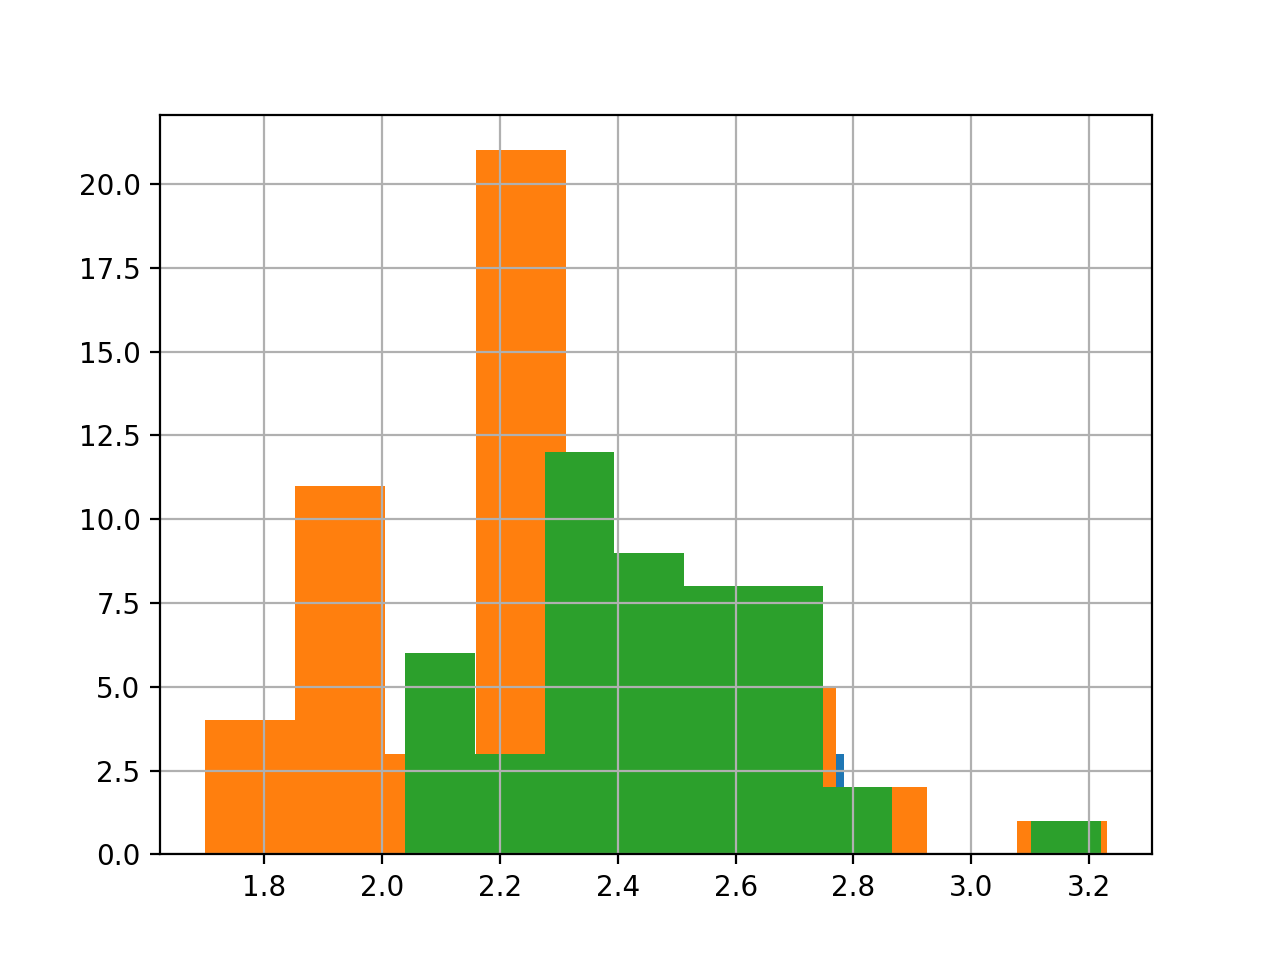
\includegraphics[width=\textwidth]{v3.png}\\
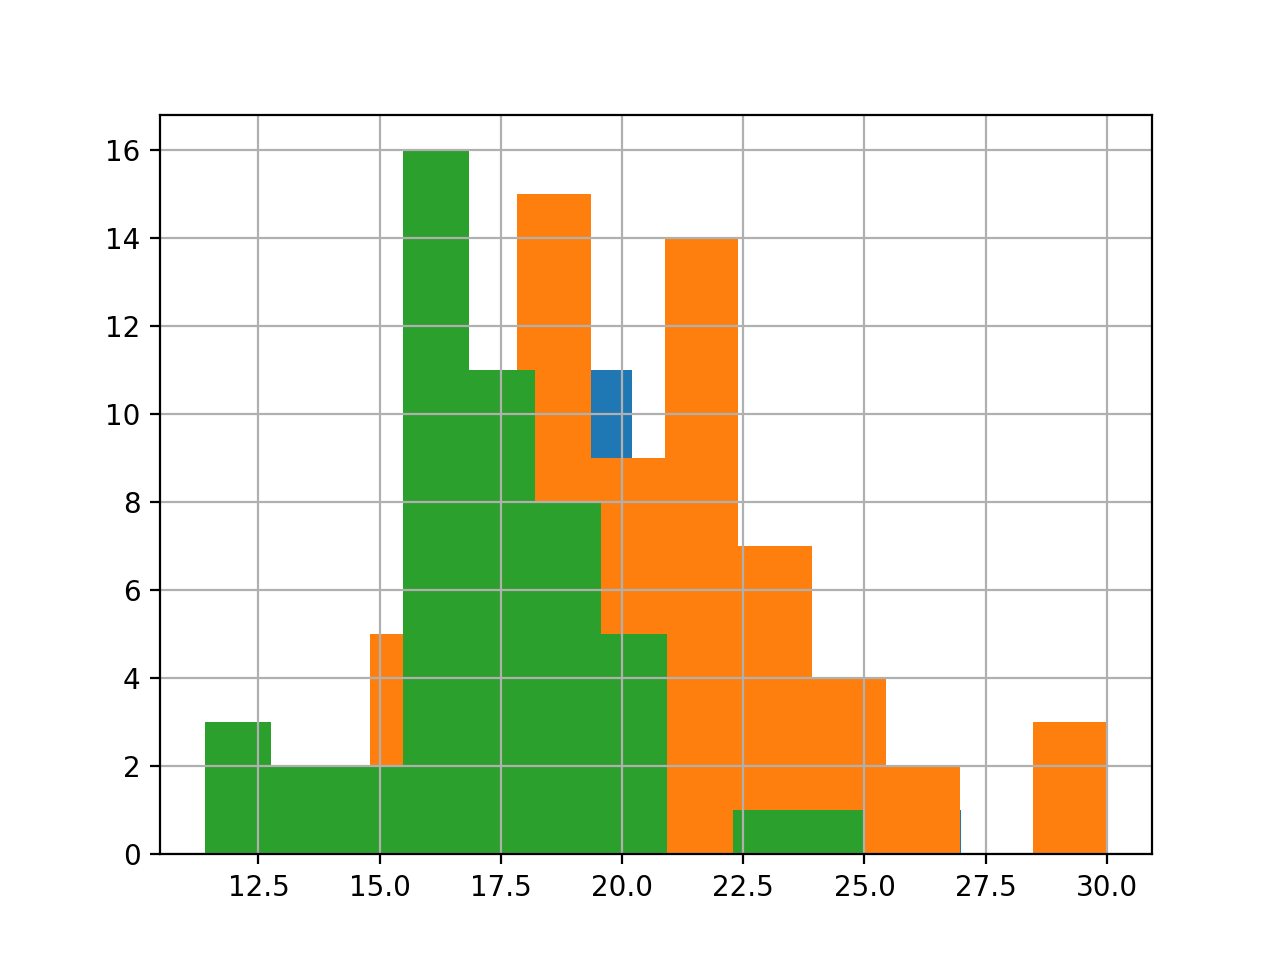
\includegraphics[width=\textwidth]{v4.png}\\
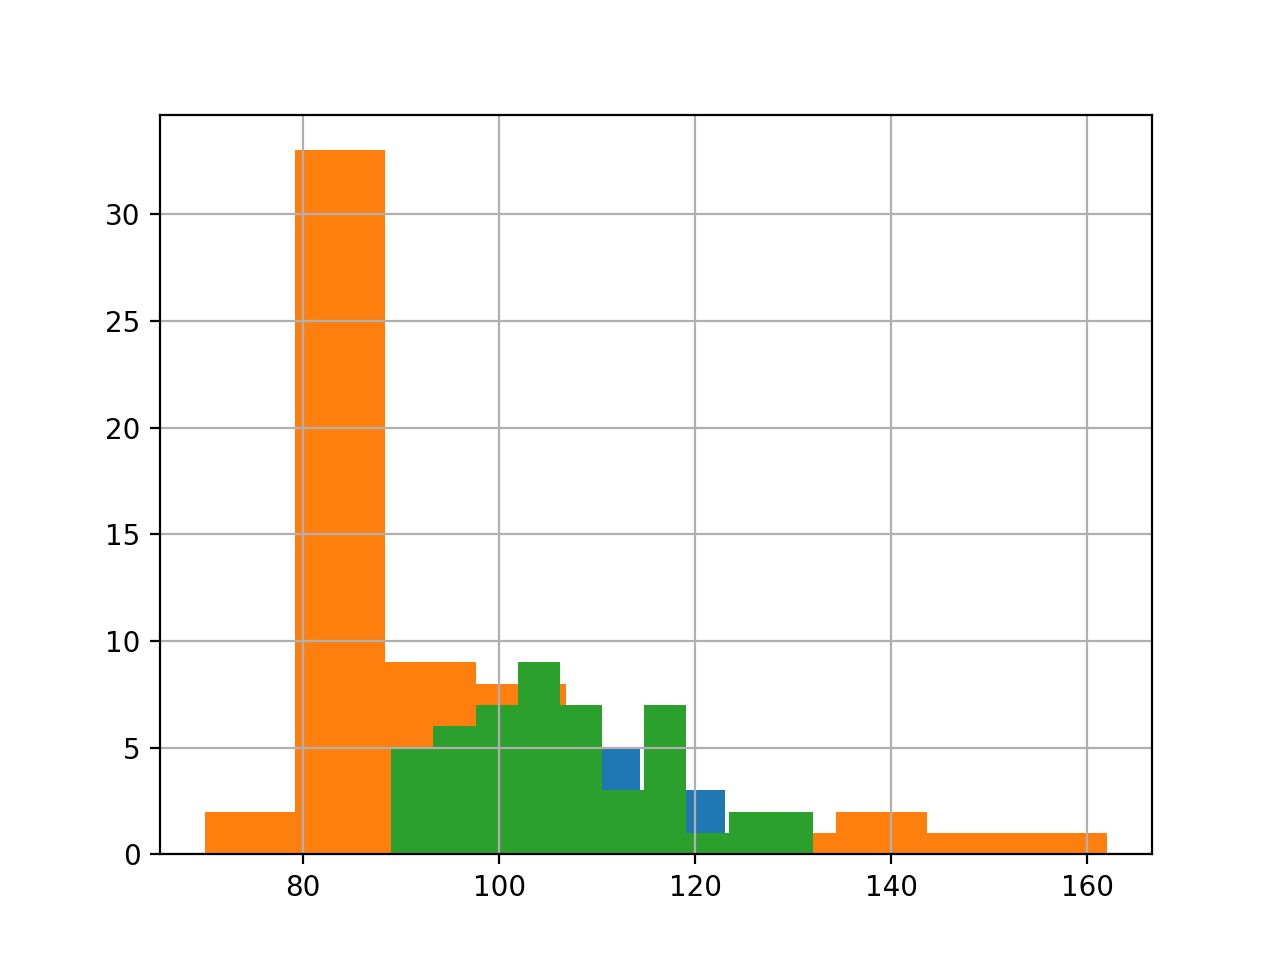
\includegraphics[width=\textwidth]{v5.png}\\
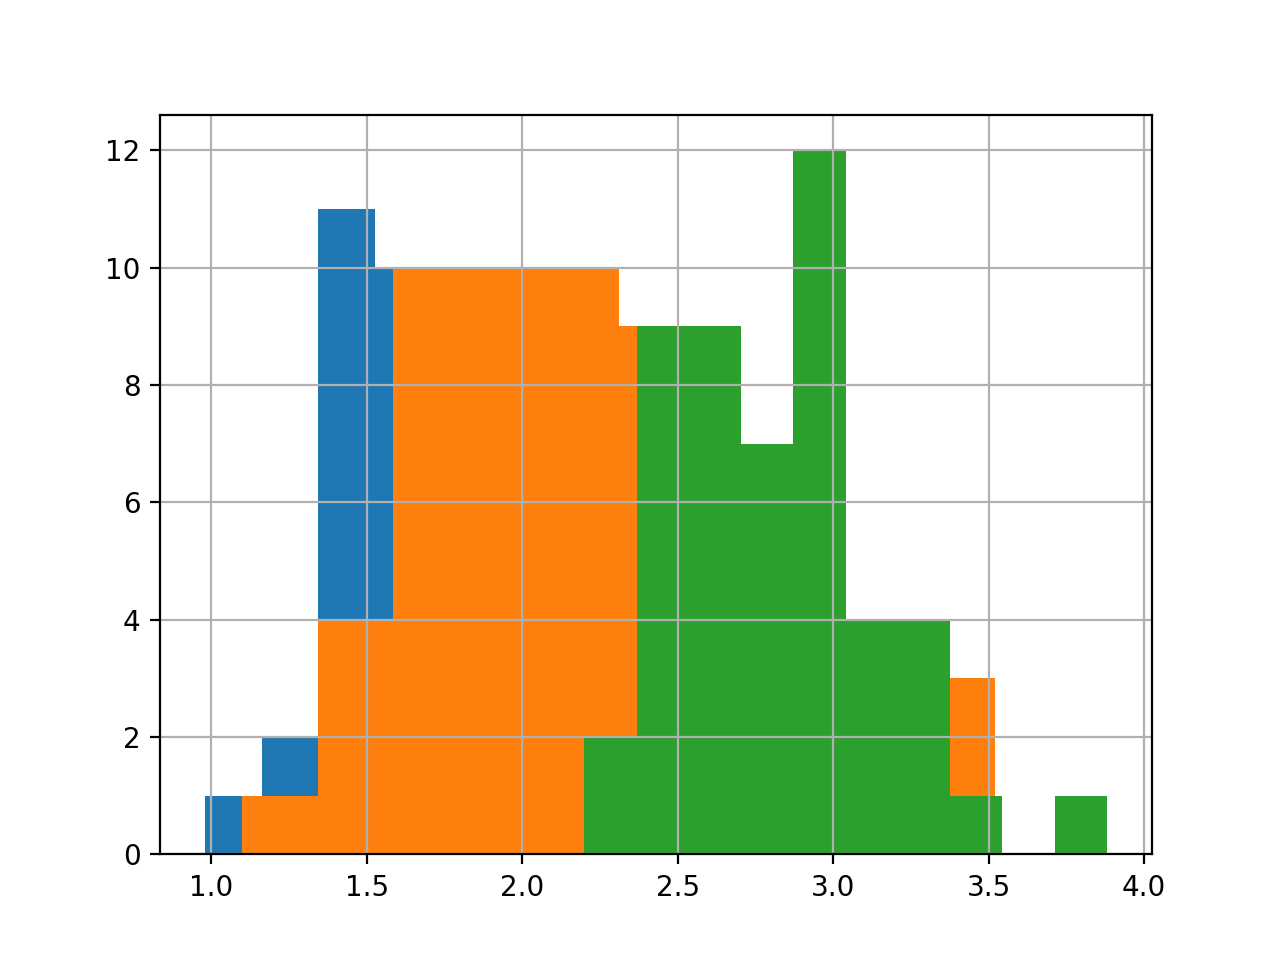
\includegraphics[width=\textwidth]{v6.png}\\
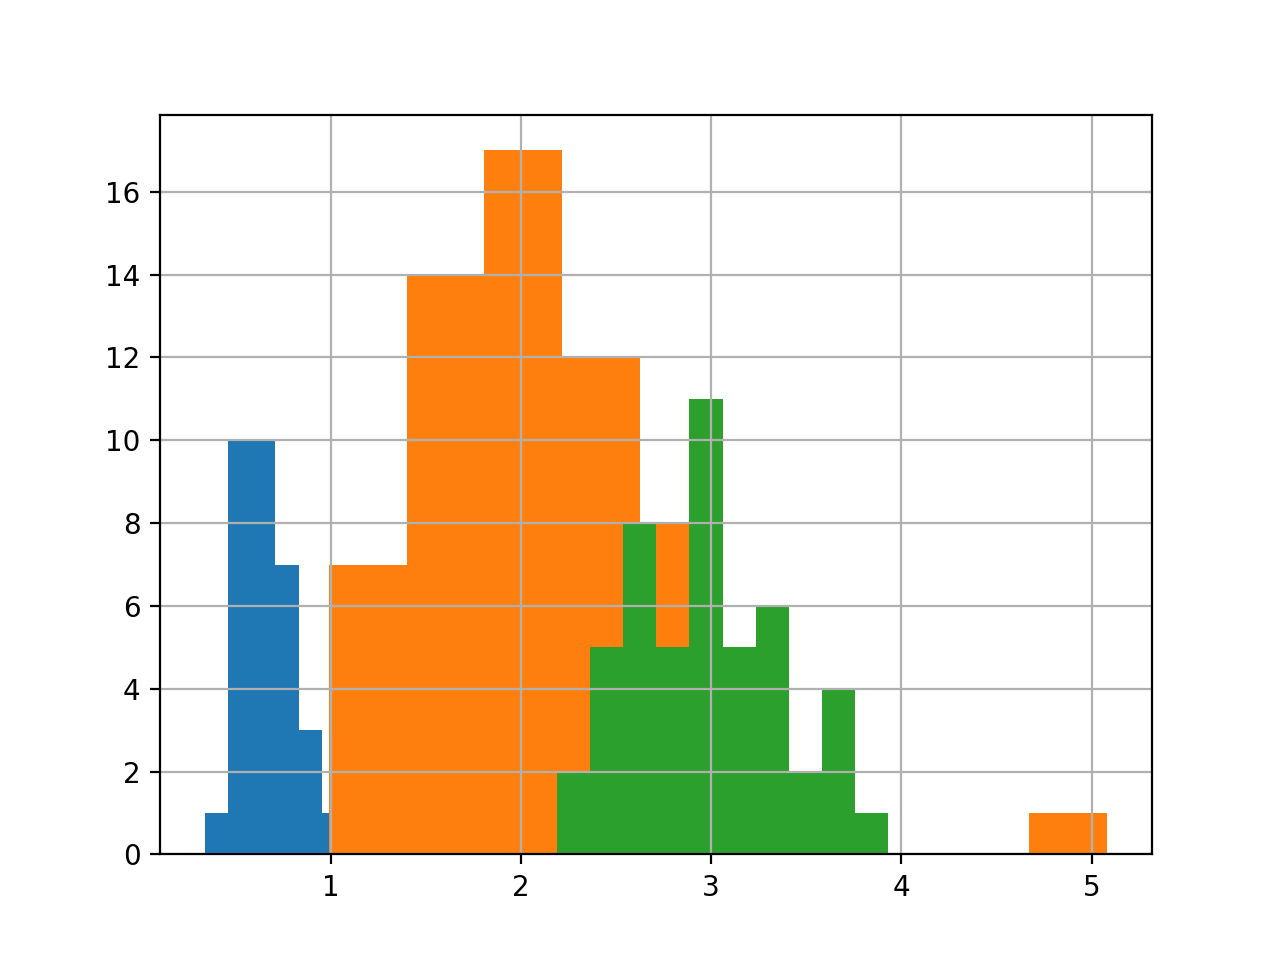
\includegraphics[width=\textwidth]{v7.png}\\
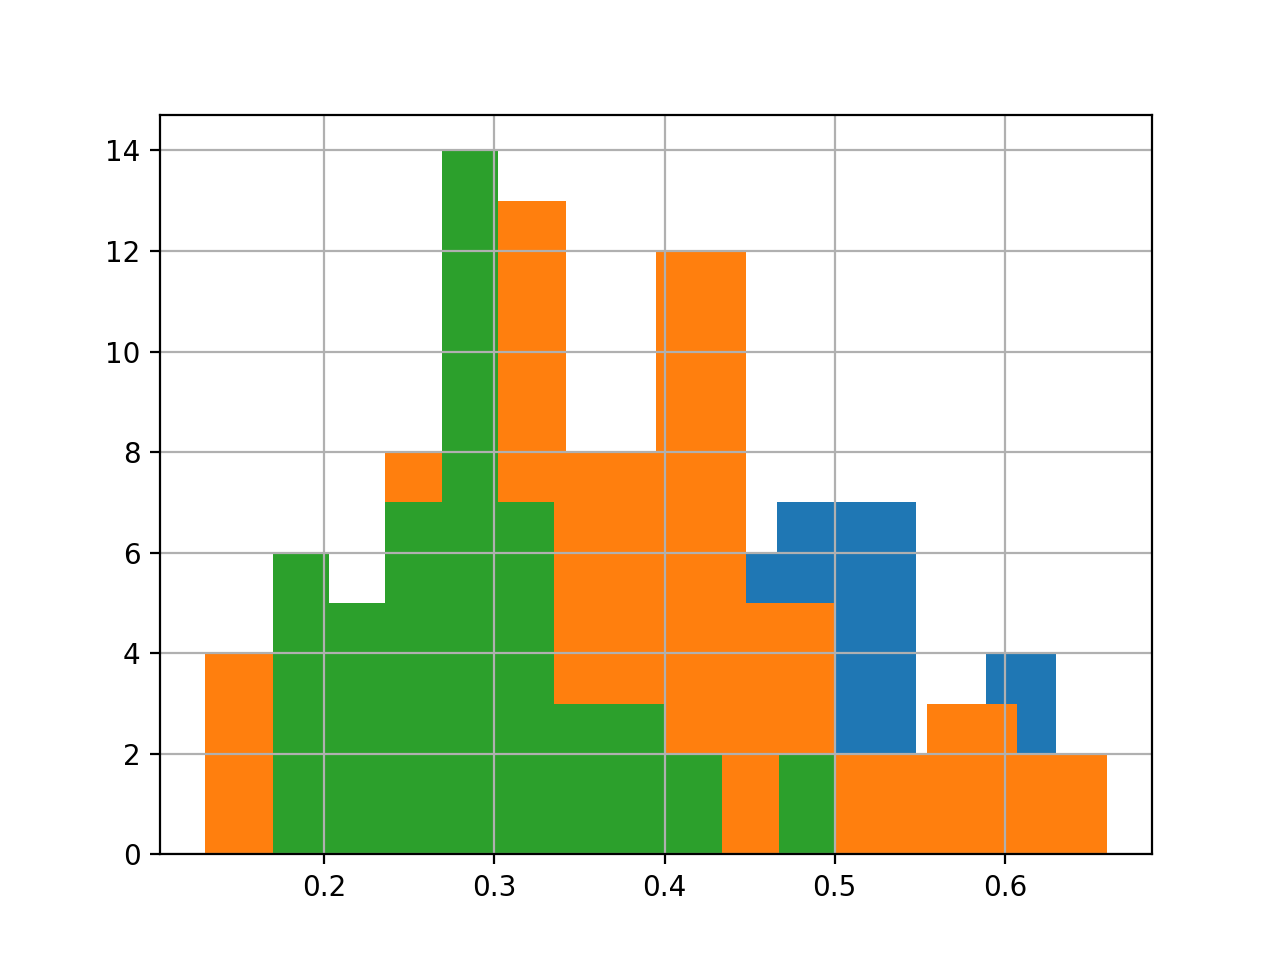
\includegraphics[width=\textwidth]{v8.png}\\
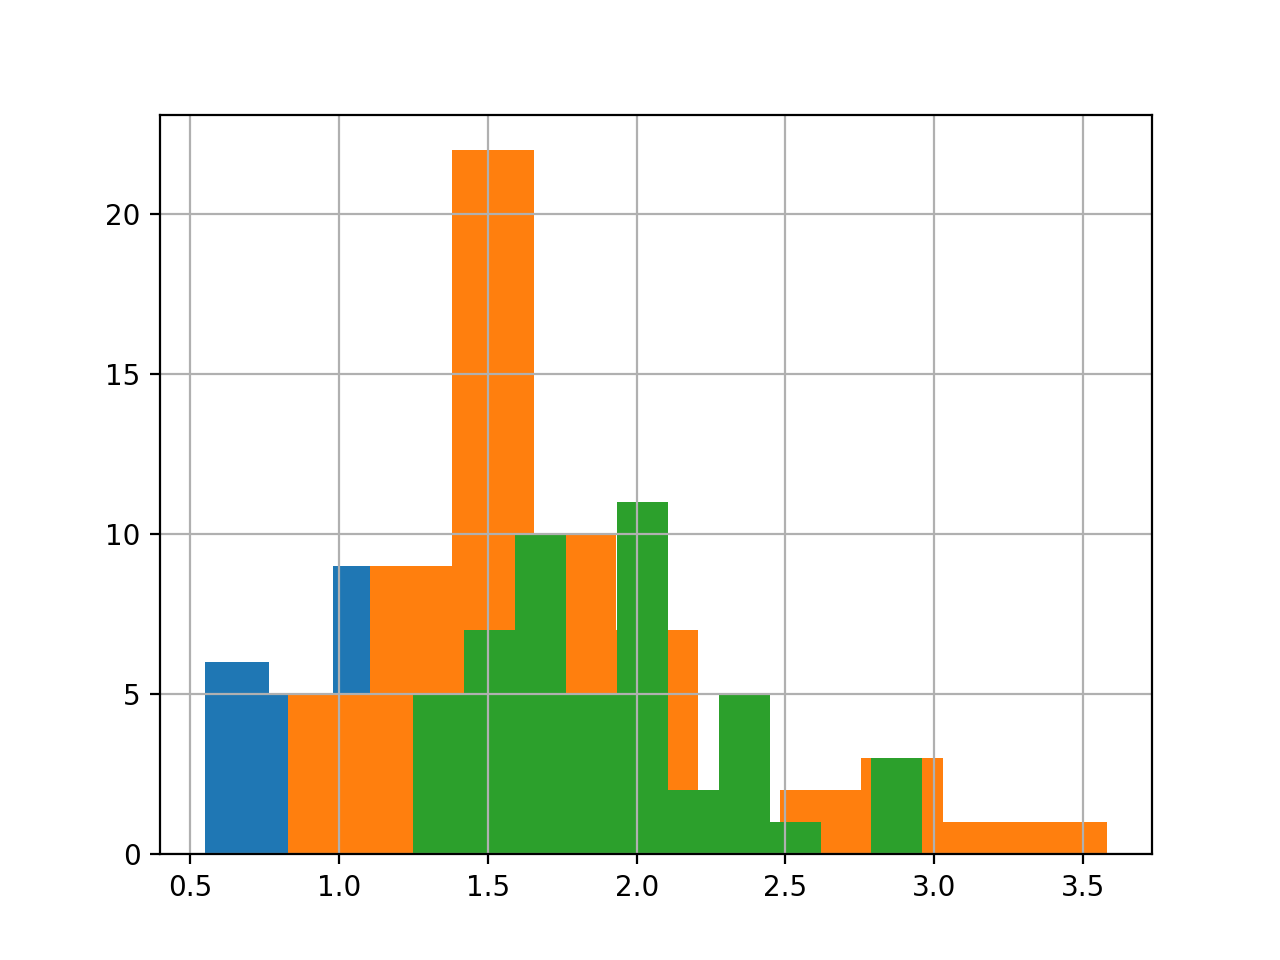
\includegraphics[width=\textwidth]{v9.png}\\
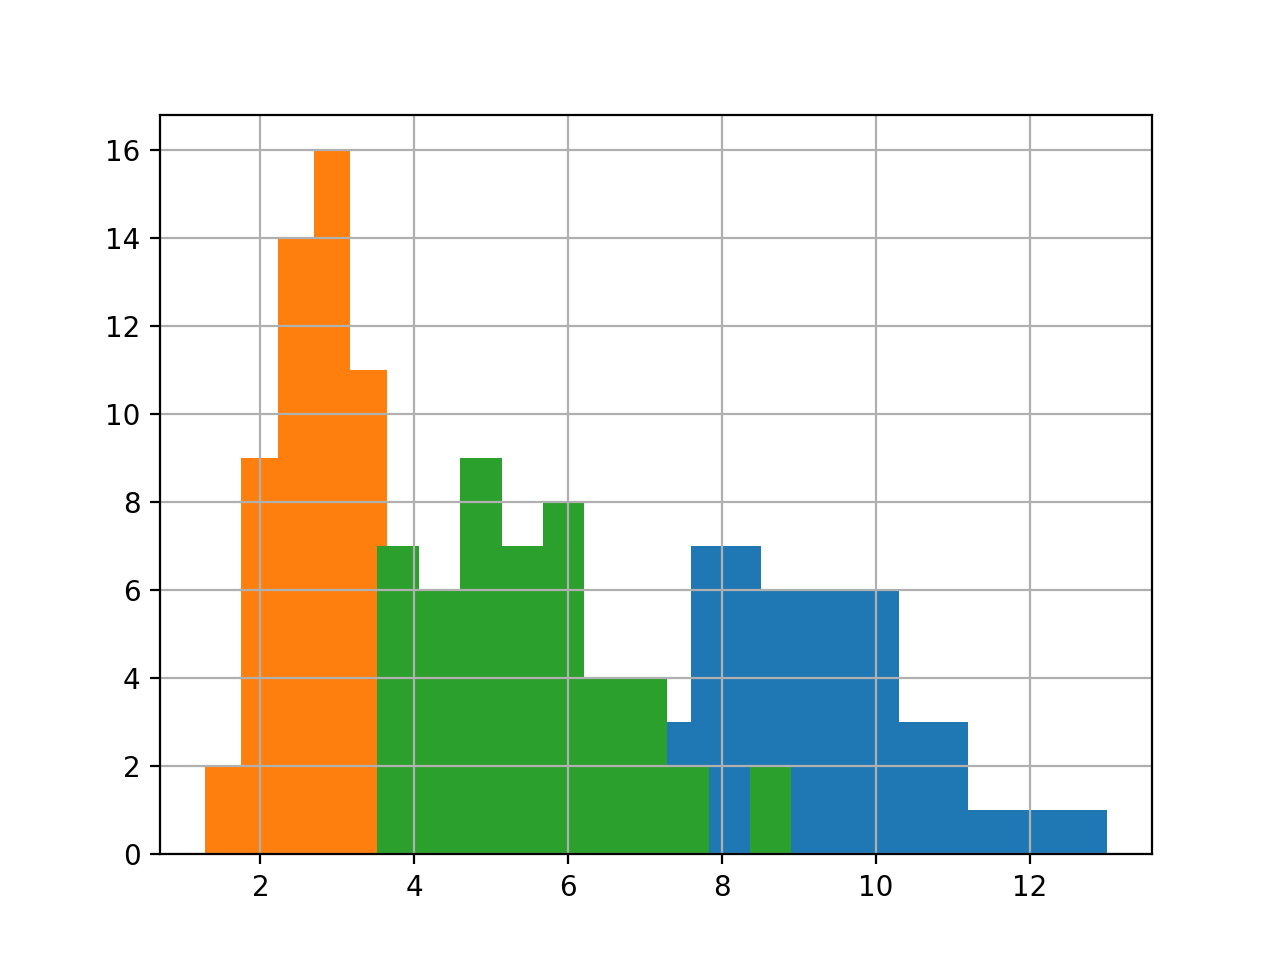
\includegraphics[width=\textwidth]{v10.png}\\
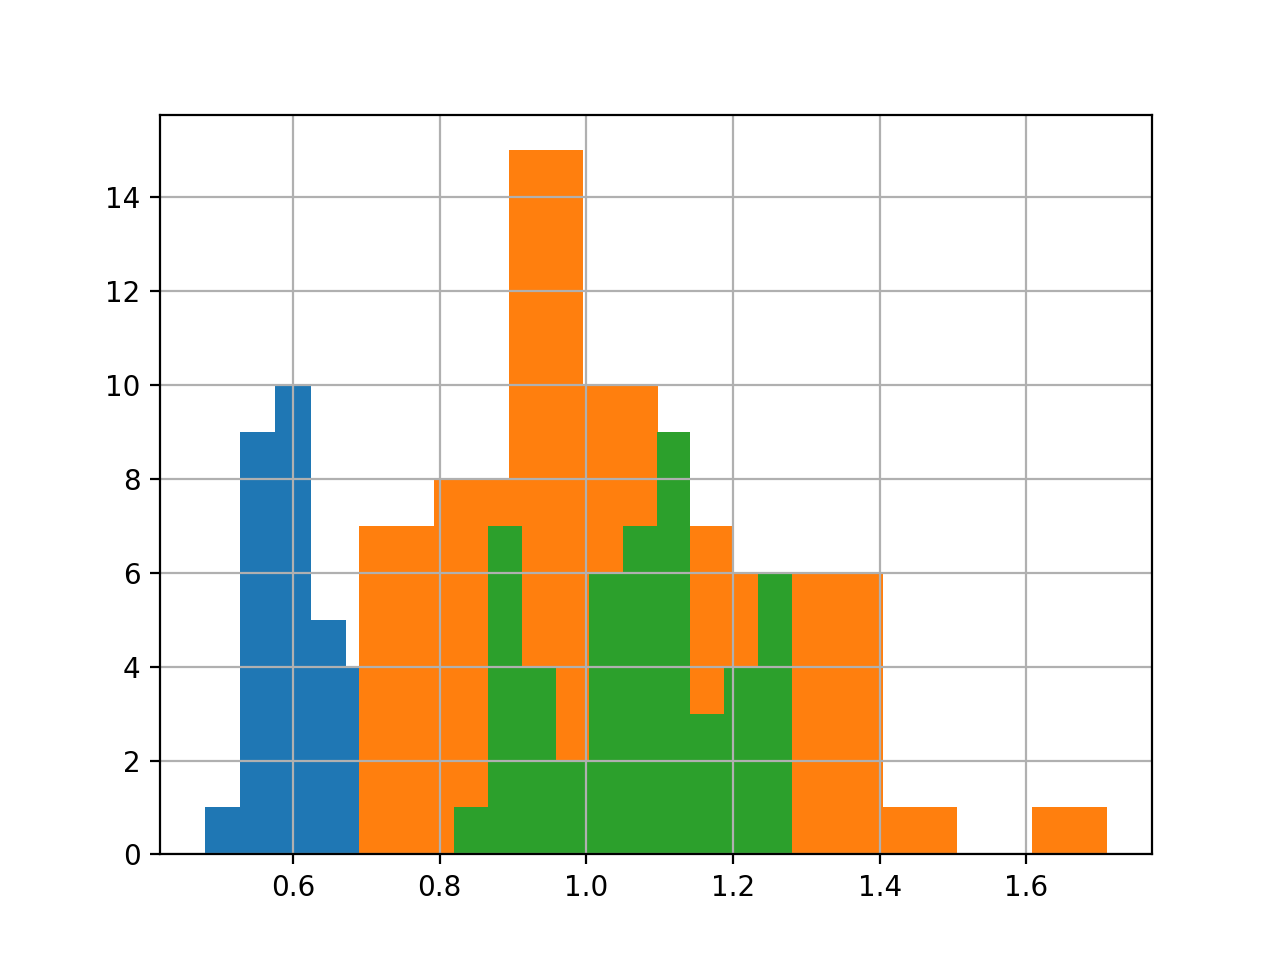
\includegraphics[width=\textwidth]{v11.png}\\
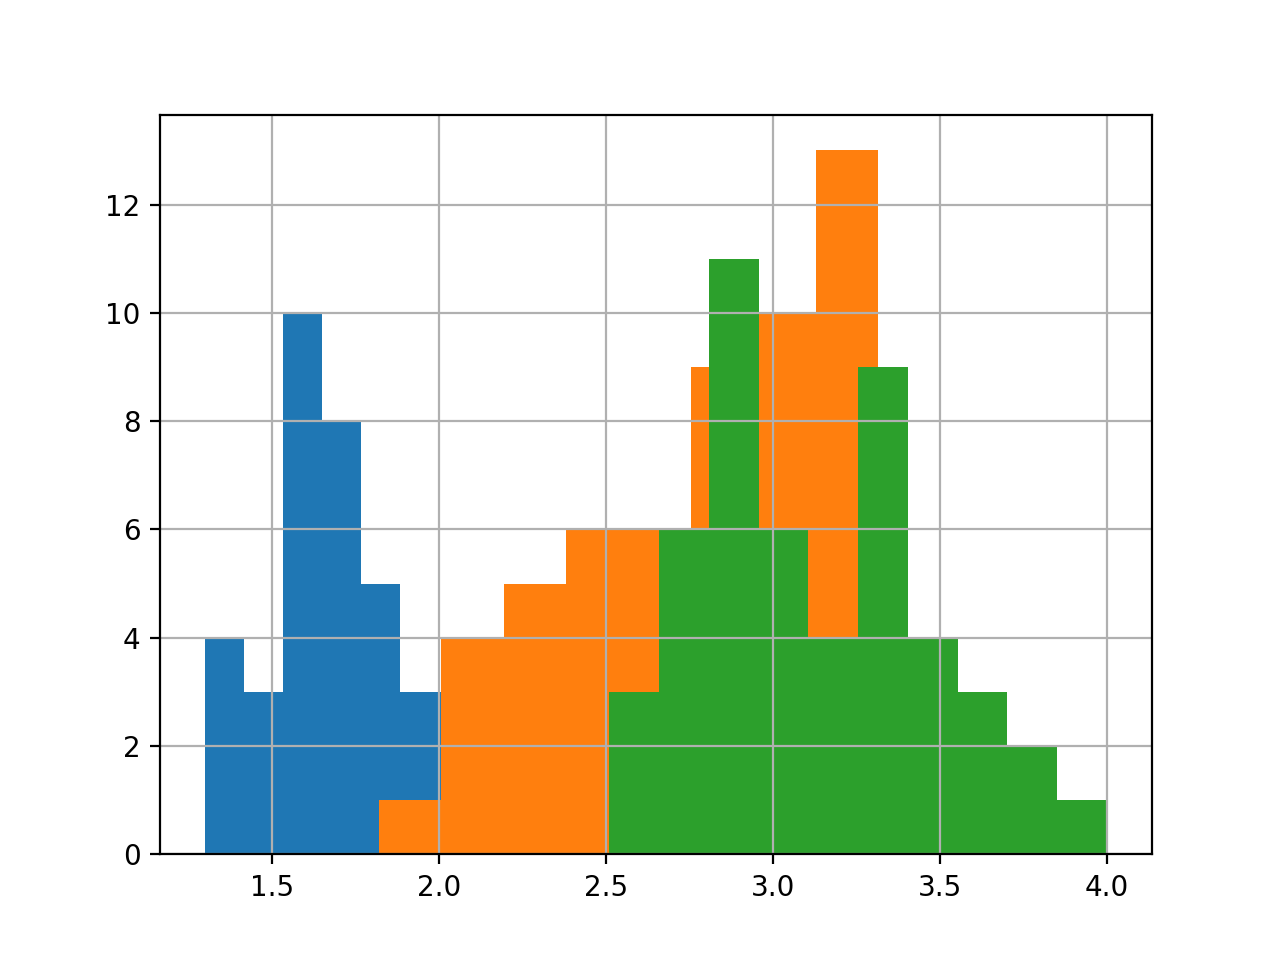
\includegraphics[width=\textwidth]{v12.png}\\
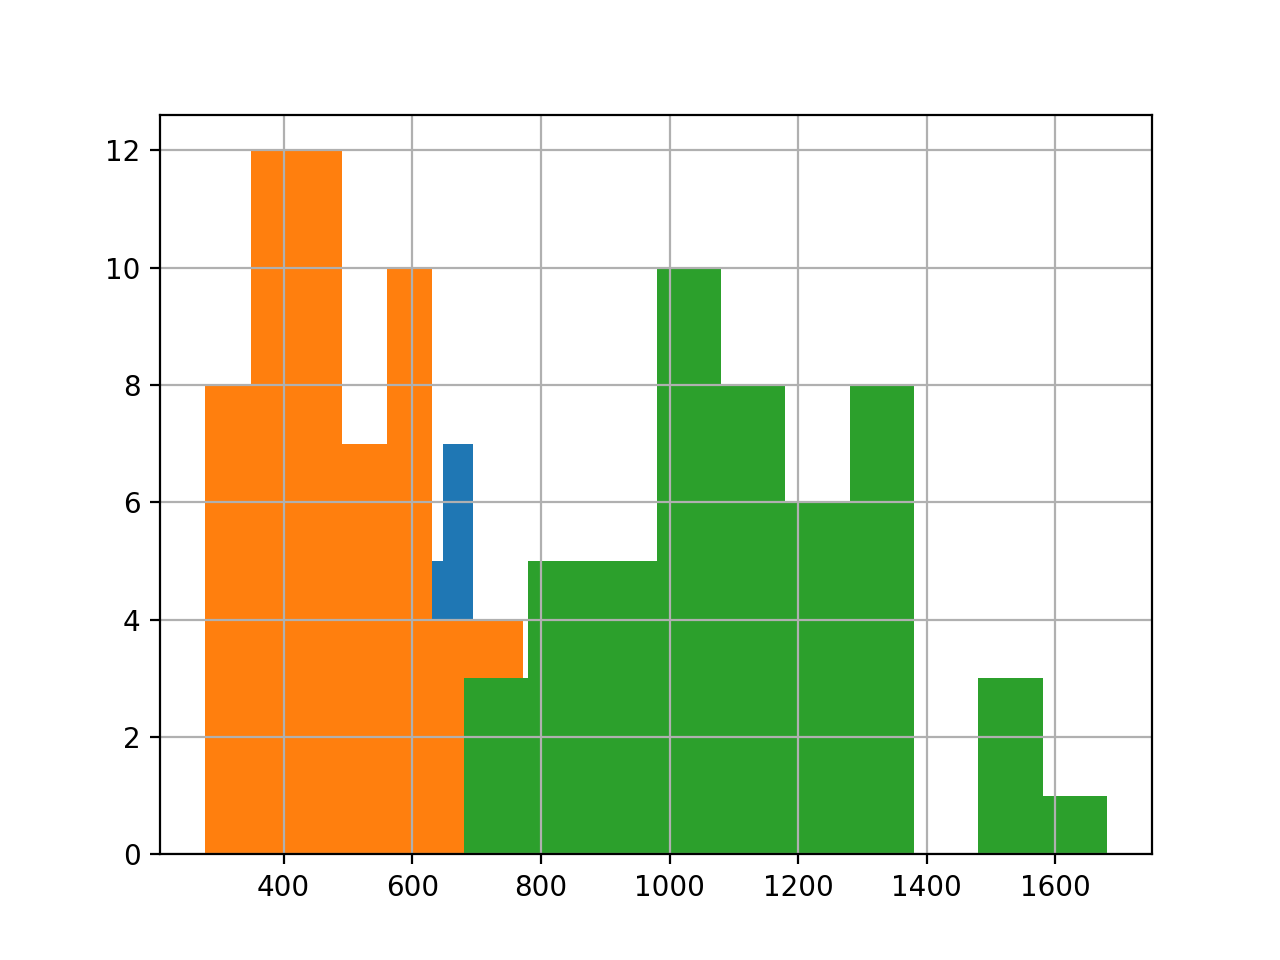
\includegraphics[width=\textwidth]{v13.png}\\

\subsubsection*{4}


\end{document}